\documentclass[10pt,a4paper]{report}
\usepackage[utf8]{inputenc}
\usepackage[spanish]{babel}
\usepackage{amsmath}
\usepackage{amsfonts}
\usepackage{amssymb}
\usepackage{makeidx}
\usepackage{graphicx}
\usepackage{titlesec}
\usepackage{sectsty}
\usepackage{listings}
\usepackage{color}
\usepackage{float}
\usepackage{hyperref}
\usepackage{apacite}

\UseRawInputEncoding

\titleformat{\chapter}[display]
{\normalfont\bfseries}{}{0pt}{\Large}
\chaptertitlefont{\Huge}

\definecolor{codegreen}{rgb}{0,0.6,0}
\definecolor{codegray}{rgb}{0.5,0.5,0.5}
\definecolor{codepurple}{rgb}{0.58,0,0.82}
\definecolor{backcolour}{rgb}{0.95,0.95,0.92}

\lstdefinestyle{mystyle}{
	backgroundcolor=\color{backcolour},   
	commentstyle=\color{codegreen},
	keywordstyle=\color{magenta},
	numberstyle=\tiny\color{codegray},
	stringstyle=\color{codepurple},
	basicstyle=\footnotesize,
	breakatwhitespace=false,         
	breaklines=true,                 
	captionpos=b,                    
	keepspaces=true,                 
	numbers=left,                    
	numbersep=5pt,                  
	showspaces=false,                
	showstringspaces=false,
	showtabs=false,                  
	tabsize=2,
	frame=lines
}

\lstset{style=mystyle}

\author{Medina Medina, David A.\\}
\title{Jena 3\\Consultando la web sem\'antica con \textit{SPARQL}}
\begin{document}
	\maketitle
	\tableofcontents
	\abstract{
	En este documento se muestran las consultas y resultados obtenidos en los diferentes ejercicios propuestos. Se utiliza para tal fin una aplicaci\'on en desarrollada en \textit{Java} para la realizaci\'on de consultas \textit{SPARQL}. 
	
	Estas consultas podr\'an realizarse en local --mediante un fichero \textit{RDF} de entrada-- o en remoto --utilizando una direcci\'on URL hacia un \textit{endpoint} desde el cual se desee realizar la consulta.
	
	El resultado de las consultas \textit{SPARQL} pueden ser visualizados desde la aplicaci\'on o almacenados un fichero local en dos posibles formatos: texto o \textit{SRX}.
	}

	\begin{figure}[H]\label{fig:gp2d12-espera}
		\centering
		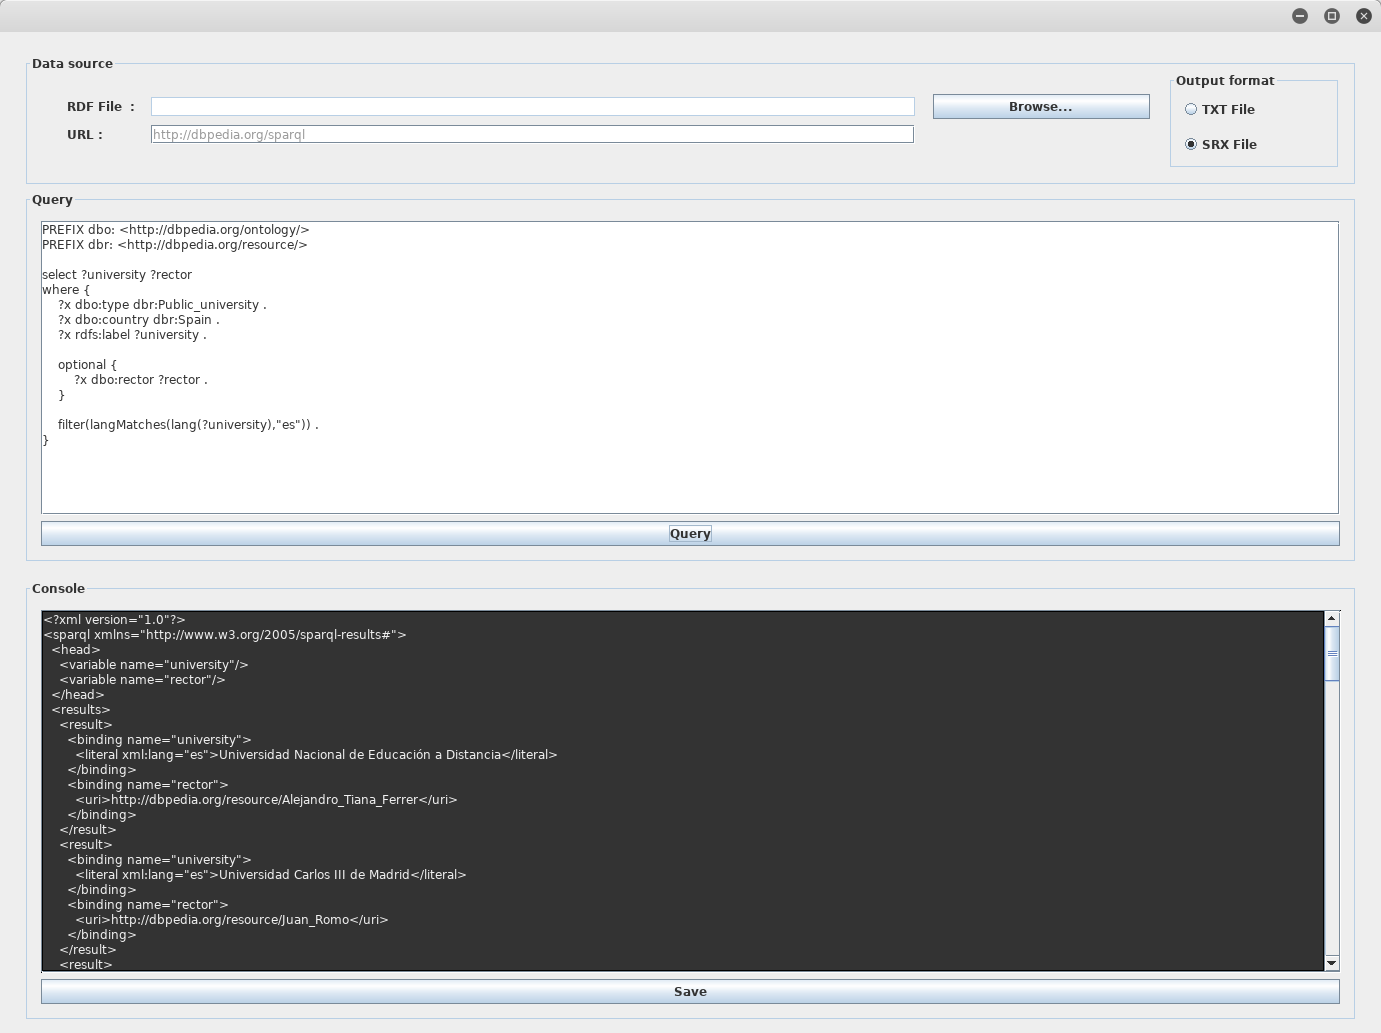
\includegraphics[width=0.75\textwidth]{aplicacion.png}
		\caption{Programa desarrollado en \textit{Java} para realizar consultas \textit{SPARQL}}
	\end{figure}
	
	
	\chapter{Consultas locales utilizando un fichero \textit{RDF}}
	\section{Obtener el n\'umero total de art\'iculos}
	
	
	\lstinputlisting[language=SQL, caption=Consulta SPARQL]{./ejercicio2/consulta2-1.txt}
	
	\lstinputlisting[language=SQL, caption=Resultado en formato \textit{TXT}]{./ejercicio2/resultado2-1.txt}
	
	\lstinputlisting[language=SQL, caption=Resultado en formato \textit{SRX}]{./ejercicio2/resultado2-1.srx}
	
	
	\section{Obtener  el  n\'umero  de  art\'iculos  para  cada  una  de  las  revistas  por  orden  creciente  de n\'umero de art\'iculos}
	
	
	\lstinputlisting[language=SQL, caption=Consulta SPARQL]{./ejercicio2/consulta2-2.txt}
	
	\lstinputlisting[language=SQL, caption=Resultado en formato \textit{TXT}]{./ejercicio2/resultado2-2.txt}
	
	\lstinputlisting[language=SQL, caption=Resultado en formato \textit{SRX}]{./ejercicio2/resultado2-2.srx}
	
	
	\section{Obtener el t\'itulo y n\'umero de autores de los art\'iculos que poseen m\'as de 8 autores por orden decreciente de n\'umero de autores}
	
	
	\lstinputlisting[language=SQL, caption=Consulta SPARQL]{./ejercicio2/consulta2-3.txt}
	
	\lstinputlisting[language=SQL, caption=Resultado en formato \textit{TXT}]{./ejercicio2/resultado2-3.txt}
	
	\lstinputlisting[language=SQL, caption=Resultado en formato \textit{SRX}]{./ejercicio2/resultado2-3.srx}
	
	
	\section{Obtener  los  10  autores  que  m\'as  art\'iculos  firman  por  orden  decreciente  de  n\'umero de art\'iculos firmados. }
	
	
	\lstinputlisting[language=SQL, caption=Consulta SPARQL]{./ejercicio2/consulta2-4.txt}
	
	\lstinputlisting[language=SQL, caption=Resultado en formato \textit{TXT}]{./ejercicio2/resultado2-4.txt}
	
	\lstinputlisting[language=SQL, caption=Resultado en formato \textit{SRX}]{./ejercicio2/resultado2-4.srx}
	
	
	
	\chapter{Consultas remotas a la \textit{URL} de \textit{DBpedia}}
	Esta consulta \textit{SPARQL} buscaremos las universidades espa\~nolas que aparecen en la DBpedia mostrando su nombre en espa\~nol y para aquellas que tiene el rector, mostrarlo tambi\'en. El \textit{endpoint} de la \textit{DBpedia} a utilizar se corresponde con la inglesa y no la espa\~nola.
	
	
	\lstinputlisting[language=SQL, caption=Consulta SPARQL]{./ejercicio3/consulta3.txt}
	
	\lstinputlisting[language=SQL, caption=Resultado en formato \textit{TXT}]{./ejercicio3/resultado3.txt}
	
	\lstinputlisting[language=SQL, caption=Resultado en formato \textit{SRX}]{./ejercicio3/resultado3.srx}
	
	
\end{document}